\documentclass{beamer}


\usepackage{listings}
\usepackage[italian]{babel}
\usepackage[T1]{fontenc}
\usepackage{beamerthemebjeldbak}
\usepackage{graphicx}
\usepackage{listings}
\usepackage[utf8]{inputenc} 
\usepackage{epsfig}  
\usepackage{amsmath} 
\usepackage{url}
\usepackage{multicol}
\usepackage{amsfonts}

\usepackage{listings}% http://ctan.org/pkg/listings
\lstset{
  basicstyle=\ttfamily,
  mathescape
}

\setbeamertemplate{itemize/enumerate body begin}{\footnotesize}

\title{Big Network Visualizzation Tool for iNSIdEnano}
\author{Luigi Giugliano}
\institute{Universit\'a degli studi di Salerno}


\begin{document}

\begin{frame}
   \maketitle
\end{frame}

\begin{frame}
  \frametitle{Overview}
  \footnotesize \tableofcontents
\end{frame}

\AtBeginSection[]
  {
     \begin{frame}<beamer>
     \frametitle{Overview}
   \footnotesize \tableofcontents[currentsection]
     \end{frame}
}


\section{iNSIdEnano}
\begin{frame}
\frametitle{iNSIdEnano}
iNSIdEnano è un tool grafico che mette in evidenza le connessioni tra entità fenotipiche del tipo:
\begin{itemize}
\item Esposizione ai nanomateriali
\item Trattamenti farmaceutici
\item Esposizione ad agenti chimici
\item Malattie
\end{itemize}
L' interazione tra queste entità è valutata in base al loro effetto sull'espressione dei geni.
\end{frame}

\begin{frame}
\begin{center}
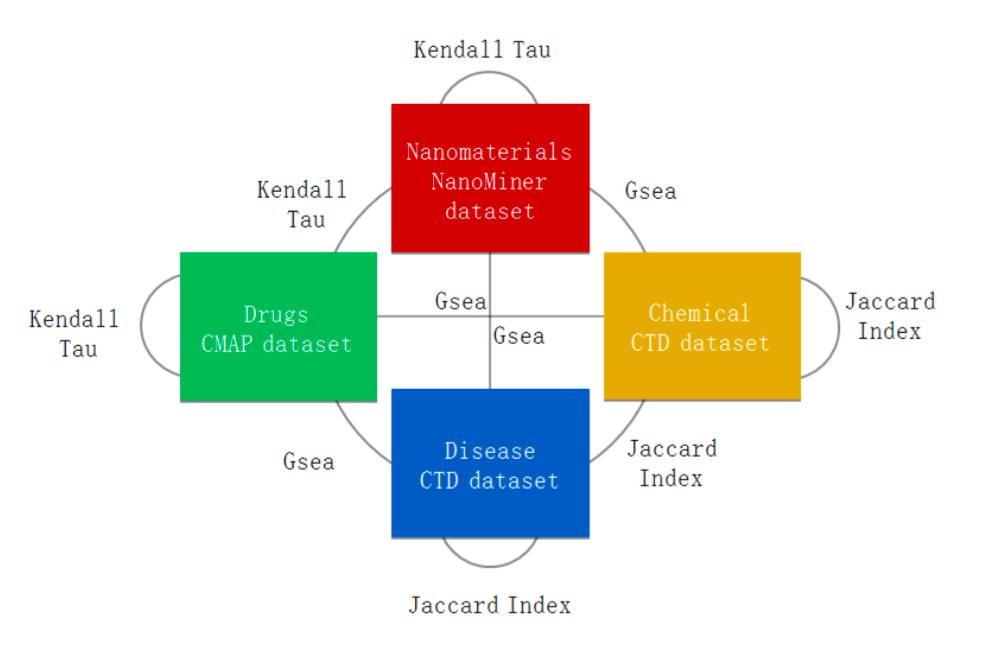
\includegraphics[scale=0.27]{img/OverviewGraph.png}
\end{center}
E' stata calcolata la distanza per ogni coppia di entità. Sono poi state normalizzate tra -1 e 1 per renderle confrontabili.
\end{frame}

\begin{frame}
Per ogni entità fenotipica nel dataset, è assegnata una lista di geni. In particolare un'insieme di geni è associato a ogni malattia e ogni agente chimico, invece per ogni farmaco e per ogni nanomateriale è associata una lista ordinata di geni. \\
\medskip
Quindi per costruire una network di similarità tra entità fenotipiche è stato necessario calcolare la similarità a coppie per ogni entità.
\end{frame}

\begin{frame}
\frametitle{Insieme di geni vs Insieme di geni}
Il Jaccard index è stato utilizzato per calcolare la similarità tra due malattie, tra due agenti chimici o tra un agente chimico e una malattia.\\
Dati due insiemi A e B l'indice di Jaccard è dato dalla dimensione della loro intersezione diviso la dimensione della loro unione.
\begin{equation}
J(A, B) = \frac{|A \cap B|}{|A \cup  B|}
\end{equation}
Questa misura è zero se i due insieme non condividono neanche un gene, mentre 1 se sono esattamente uguali.\\
Per ogni agente chimico vengono considerati due set di geni: quelli che sono up-regolati da quell'agente chimico e quelli che sono down-regolati.
Per quelli down-regolati il Jaccard index è calcolato con il segno negativo.
\end{frame}


\begin{frame}
\frametitle{Insieme di geni vs Insieme di geni}
La distanza Kendall Tau è stata utilizzata per calcolare la similarità tra nanomateriali e nanomateriali, tra farmaci e farmaci e tra nanomateriali e farmaci, basata sulla lista ordinata dei geni.
La distanza Kendall Tau tra due liste $T1$ e $T2$ è definita come segue:
\begin{equation}
K(T_1, T_2) = |(i, j): i < j, (T_1(i) < T_1(i) \wedge  T_2(i) > T_2(j)) \vee
\end{equation}
\begin{center}$
 (T_1(i) > T_i(j) \wedge T_2(i) < T_2(J))  |
$
\end{center}
questa distanza è compresa tra 0 e $n(n$ $1)$, dove $n$ è la lunghezza della lista. Il valore significa che gli elementi nella lista sono nello stesso ordine, mentre il valore $n(n$ $1)$, indica che gli elementi sono in ordine opposto
\end{frame}


\section{Problema}
\begin{frame}
.
\end{frame}

\section{Soluzione}
\begin{frame}
.
\end{frame}

\end{document}